\documentclass[11pt]{article}
\usepackage[T1]{fontenc}
\usepackage[utf8]{inputenc}
\usepackage{graphicx}
\usepackage{minitoc}
\usepackage[french]{babel}
\usepackage[right=2.5cm, bottom=2.5cm,top=2.5cm, left=2.5cm]{geometry}
\title{\vspace{\fill} Cryptographie et sécurité \\ ~\textbf{IFT-606} \\~\\ Devoir 1 - Cryptographie et attaques}
\author{Amandine Fouillet - 14 130 638 ~\\ Frank Chassing - 14 153 710}
\date{\today \vspace{\fill}}

\begin{document}
\maketitle
\newpage \thispagestyle{empty}
\null
\newpage
\tableofcontents
\listoffigures
\newpage
\section{Wi-Fi}
\subsection{Fonctionnement des trois algorithmes de chiffrement}
\subsection{Points faibles et attaques possibles des trois algorithmes de chiffrement}
\subsection{Aircrack-ng}
\newpage
\section{Chiffrement et signature}
\subsection{Génération d'une paire de clé RSA}
Pour générer une paire de clé RSA d'une taille de 2048 bits protégée par un mot de passe, on exécute la commande suivante : \textit{genrsa -out cle.pem -des 2048} (\ref{fig:gen}). Le fichier généré cle.pem (\textsc{Figure \ref{fig:cle}}) contient maintenant la paire de clé RSA d'une taille de 2048.
\begin{figure}[hbtp]
    \begin{minipage}[b]{0.4\linewidth}
        \centering 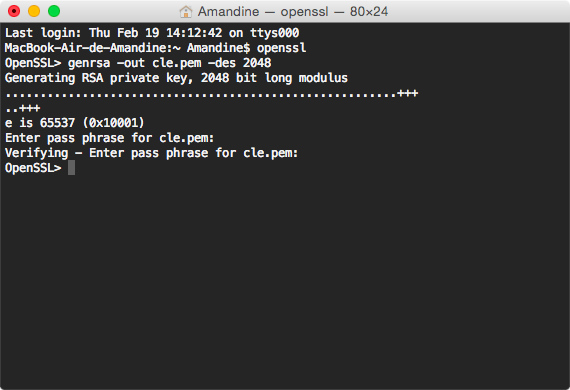
\includegraphics[scale=0.4]{Capture/question1.png}
        \caption{Génération de la paire}
                \label{fig:gen}
\label{fig:base}
    \end{minipage}\hfill
    \begin{minipage}[b]{0.48\linewidth}
        \centering 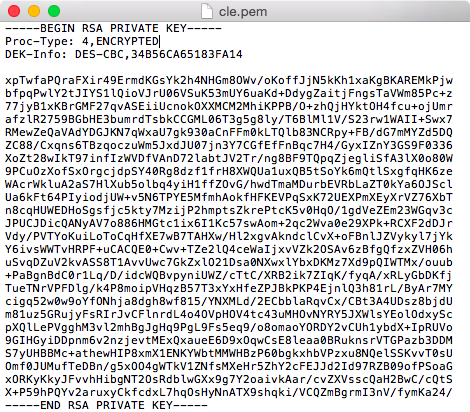
\includegraphics[scale=0.4]{Capture/question1b.png}
        \caption{Fichier obtenu}
         \label{fig:cle}
    \end{minipage}
\end{figure}

\subsection{Création d'un fichier contenant la partie publique de la clé RSA}
Pour créer un fichier contenant seulement la partie publique de la clé RSA on exécute la commande suivante : \textit{rsa -in cle.pem -pubout -out clePublique.pem} (\textsc{Figure \ref{fig:cde1}}). Le fichier généré clePublique.pem (\textsc{Figure \ref{fig:clepu}}) contient maintenant la clé publique.
\begin{figure}[hbtp]
    \begin{minipage}[b]{0.4\linewidth}
        \centering 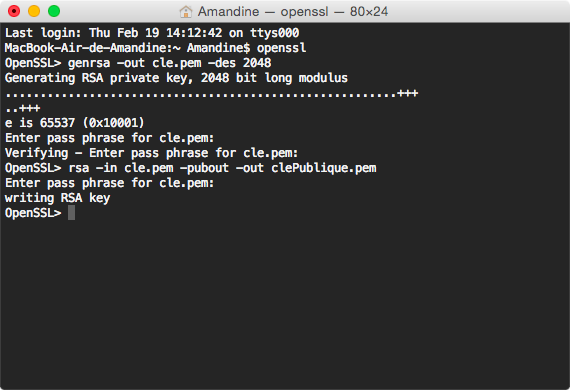
\includegraphics[scale=0.4]{Capture/question2.png}
        \caption{Exécution de la commande}
                \label{fig:cde1}
\label{fig:base}
    \end{minipage}\hfill
    \begin{minipage}[b]{0.48\linewidth}
        \centering 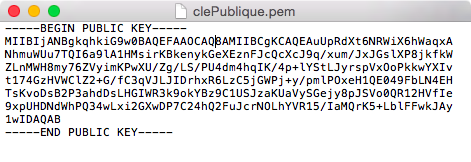
\includegraphics[scale=0.4]{Capture/question2b.png}
        \caption{Clé publique}
         \label{fig:clepu}
    \end{minipage}
\end{figure}

\subsection{Chiffrement de la partie privée générée}
Pour chiffrer la partie privée générée, on exécute la commande suivante : \textit{rsa -in cle.pem -des3 -out cle.pem}  (\textsc{Figure \ref{fig:cde2}}). Quand on réouvre le fichier cle.pem on remarque que le chiffrement a changé pour un chiffrement avec l'algorithme des3 (\textsc{Figure \ref{fig:clep}}).

\begin{figure}[hbtp]
    \begin{minipage}[b]{0.4\linewidth}
        \centering 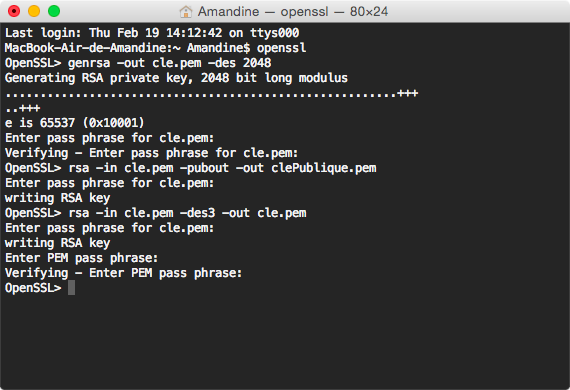
\includegraphics[scale=0.4]{Capture/question3.png}
        \caption{Exécution de la commande}
                \label{fig:cde2}
\label{fig:base}
    \end{minipage}\hfill
    \begin{minipage}[b]{0.48\linewidth}
        \centering 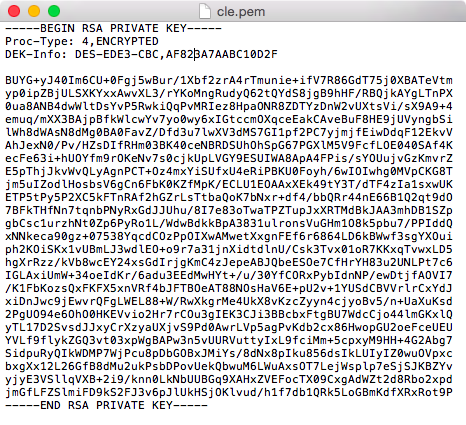
\includegraphics[scale=0.4]{Capture/question3b.png}
        \caption{Fichier cle.pem}
         \label{fig:clep}
    \end{minipage}
\end{figure}

\subsection{Chiffrement d'un message}
Nous allons maintenant chiffrer le fichier message.txt (\textsc{Figure \ref{fig:message}}) qui contient le message "OpenSSL is really cool!!!". Pour se faire, nous exécutons la commande suivante : \textit{rsautl -encrypt -in message.txt -inkey cle.pem -out messageC.txt} (\textsc{Figure \ref{fig:cde3}}). Le fichier messageC.txt contient le message crypté (\textsc{Figure \ref{fig:crypt}}).
\begin{figure}[hbtp]
    \begin{minipage}[b]{0.4\linewidth}
        \centering 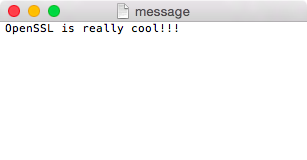
\includegraphics[scale=0.4]{Capture/question4.png}
        \caption{Fichier message.txt}
                \label{fig:message}
\label{fig:base}
    \end{minipage}\hfill
    \begin{minipage}[b]{0.48\linewidth}
        \centering 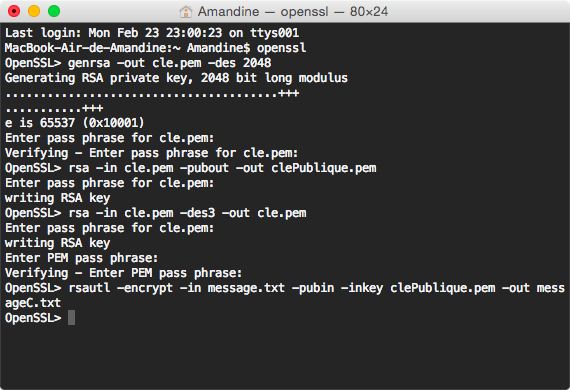
\includegraphics[scale=0.4]{Capture/question4b.png}
        \caption{Exécution de la commande}
         \label{fig:cde3}
    \end{minipage}
\end{figure}

\begin{figure}[hbtp]
        \centering 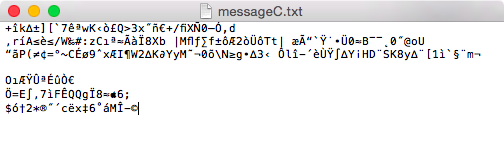
\includegraphics[scale=0.4]{Capture/question4c.png}
        \caption{Fichier messageC.txt}
         \label{fig:crypt}
\end{figure}

\subsection{Déchiffrement d'un message}
Pour déchiffrer le message du fichier messageC.txt, on exécute la commande suivante : \textit{rsautl -decrypt -in messageC.txt -inkey cle.pem -out messageD.txt} (\textsc{Figure \ref{fig:cde4}}). On obtient le fichier messageD.txt qui contient le message décrypté (\textsc{Figure \ref{fig:decrypt}}) qui correspond bien au message initial.

\begin{figure}[hbtp]
    \begin{minipage}[b]{0.4\linewidth}
        \centering 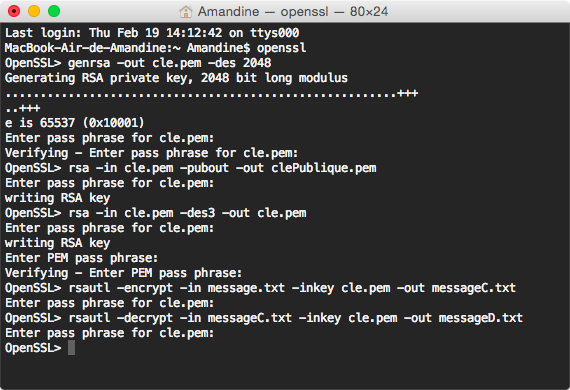
\includegraphics[scale=0.4]{Capture/question5.png}
        \caption{Exécution de la commande}
                \label{fig:cde4}
\label{fig:base}
    \end{minipage}\hfill
    \begin{minipage}[b]{0.48\linewidth}
        \centering 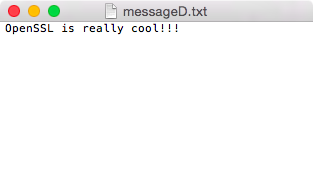
\includegraphics[scale=0.4]{Capture/question5b.png}
        \caption{Fichier messageD.txt}
         \label{fig:decrypt}
    \end{minipage}
\end{figure}
\newpage
\subsection{Signature du fichier}
Pour signer le fichier, on exécute la commande suivante : \textit{rsautl -sign -inkey cle.pem -in messageD.txt -out fic.sig} (\textsc{Figure \ref{fig:cde5}}). La  \textsc{Figure \ref{fig:signature}} montre le fichier fic.sig obtenu.
\begin{figure}[hbtp]
    \begin{minipage}[b]{0.4\linewidth}
        \centering 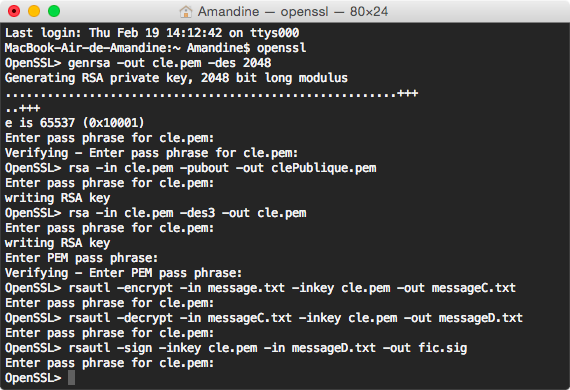
\includegraphics[scale=0.4]{Capture/question6.png}
        \caption{Exécution de la commande}
                \label{fig:cde5}
\label{fig:base}
    \end{minipage}\hfill
    \begin{minipage}[b]{0.48\linewidth}
        \centering 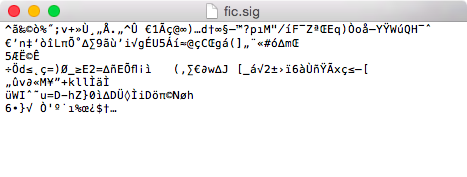
\includegraphics[scale=0.4]{Capture/question6b.png}
        \caption{Fichier fic.sig}
         \label{fig:signature}
    \end{minipage}
\end{figure}

Pour vérifier la signature, on exécute la commande suivante : \textit{rsautl -verify -pubin -inkey clePublique.pem -in fic.sig} (\textsc{Figure \ref{fig:verification}}). On obtient le résultat attendu. 
    \begin{figure}[hbtp]
        \centering 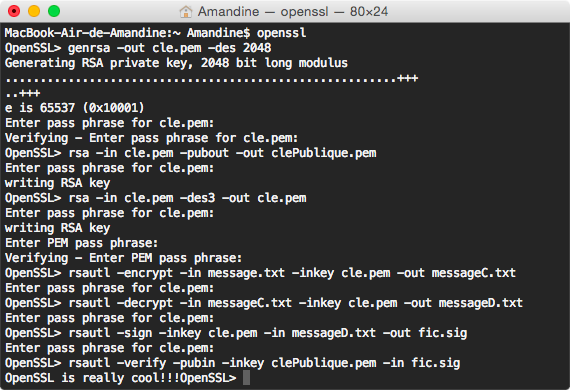
\includegraphics[scale=0.4]{Capture/question6c.png}
        \caption{Vérification de la signature}
         \label{fig:verification}
\end{figure}
\newpage
\section{Attaque décortiquée}

\end{document}